%----------------------------------------------------------------------------------------
%	PACKAGES AND THEMES
%----------------------------------------------------------------------------------------

\documentclass[aspectratio=169]{beamer}
\mode<presentation> {

	\usetheme{Boadilla}
}
\definecolor{lmugreen}{RGB}{0, 136, 58}
\usecolortheme[named=lmugreen]{structure}
\usepackage{graphicx} % Allows including images
\usepackage{booktabs} % Allows the use of \toprule, \midrule and \bottomrule in tables
\usepackage[english]{babel}
\usepackage[utf8]{inputenc}
\usepackage{amsmath,amssymb} % math symbols
\usepackage{float}
\usepackage{colortbl}
\usepackage{float}
\usepackage{hyperref} % for URLs
\usepackage{xcolor}
\definecolor{lightgray}{gray}{0.9}
\usepackage{verbatim}
\usepackage{textpos} % logo position
\usepackage[default]{sourcesanspro} % font type
\usepackage{cases} % math cases

% Caption
\usepackage{caption}
\DeclareCaptionFont{tiny}{\tiny}
\captionsetup{font=scriptsize,labelfont=scriptsize,justification=centering}

% ToC
\AtBeginSection[]{
	\begin{frame}[noframenumbering, plain]
	\frametitle{Outline}
	\setcounter{tocdepth}{1}
	\tableofcontents[currentsection]
\end{frame}
}

% Remove navigation
\beamertemplatenavigationsymbolsempty

% R
\usepackage{listings}
\lstset{
language=R,
basicstyle=\scriptsize\ttfamily,
commentstyle=\ttfamily\color{gray},
backgroundcolor=\color{white},
showspaces=false,
showstringspaces=false,
showtabs=false,
tabsize=2,
captionpos=b,
breaklines=false,
breakatwhitespace=false,
title=\lstname,
escapeinside={},
keywordstyle={},
morekeywords={},
belowskip = -1.2 \baselineskip,
}

%----------------------------------------------------------------------------------------
%	TITLE PAGE
%----------------------------------------------------------------------------------------

\addtobeamertemplate{frametitle}{}{%
	\begin{textblock*}{100mm}(0.88\textwidth,-0.5cm)
		
\includegraphics[height=1cm,width=2cm]{lmu_logo}
\end{textblock*}}

%
\includegraphics[width=0.3\textwidth]{lmu_logo}
\vspace*{-1cm}

\title{From Snapshots to Streams: A Live State Graph Approach for LLM-Based Root-Cause-Analysis in Kubernetes}

\author{OliverStempel}
\institute[LMU]{LMU}
\begin{document}

\usebackgroundtemplate{
\includegraphics[width=\paperwidth]{lmu-background.pdf}}
\begin{frame}
\begin{columns}
	\begin{column}{0.4\textwidth}
		\vspace{3cm}

		\textbf{\textcolor{white}{\Large Continuous From Snapshots to Streams: A Live State Graph Approach for LLM-Based Root-Cause-Analysis in Kubernetes }}
		\vspace{1cm}

		\textcolor{white}{\footnotesize OliverStempel \\
			\today}
	\end{column}
	\begin{column}{0.49\textwidth}
		\vspace{2cm}
		\begin{center}
			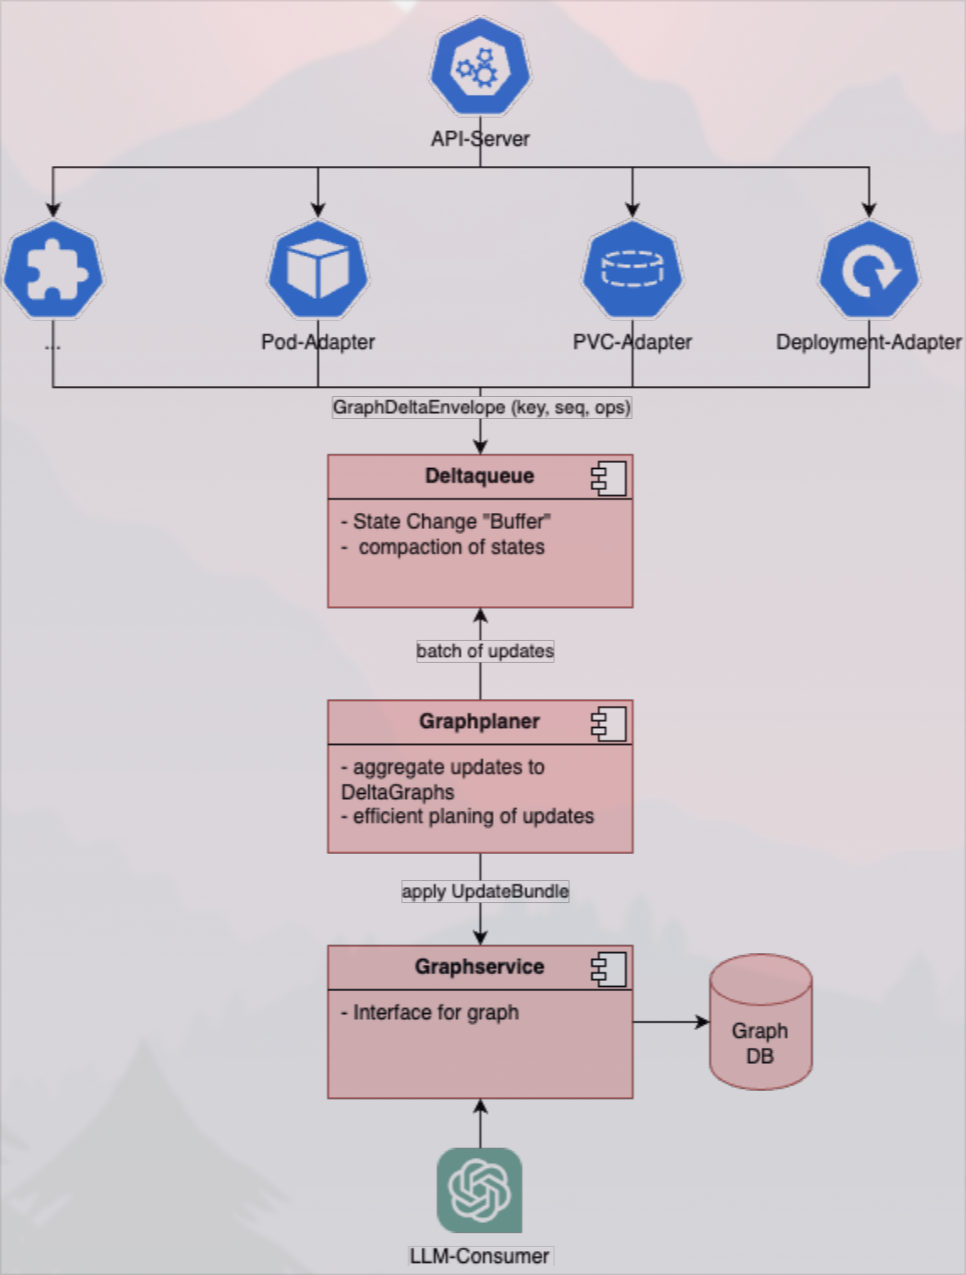
\includegraphics[width=0.5\textwidth]{architecture.png}
		\end{center}
	\end{column}
\end{columns}
\end{frame}
%----------------------------------------------------------------------------------------
%	PRESENTATION SLIDES
%----------------------------------------------------------------------------------------


\section{Introduction}

\begin{frame}{Introduction}

Example citation \cite{bischl2015}

\end{frame}

\section{Background}

\begin{frame}{Background}

Example citation \cite{bischl2015}

\end{frame}


\begin{frame}[allowframebreaks]
        \frametitle{References}
        \bibliographystyle{plain}
        \bibliography{literature.bib}
\end{frame}

\end{document}
